\hypertarget{introduction}{%
\section{Introduction}\label{introduction}}

Power-converter efficiency, thermal margin, and magnetic-component
sizing depend on models for volumetric core loss and complex
permeability. Vendor curves provide essential design information, but
cover a finite set of frequencies, flux densities, and temperatures and
normally do not provide a joint parameter distribution. Fitting one
nominal curve can therefore hide parameter non-identifiability and model
discrepancy.

Bayesian calibration represents uncertainty in model parameters
conditional on the selected model, observations, and prior. Bayesian
experimental design ranks a candidate measurement by its expected
reduction of posterior uncertainty~\citep{chaloner1995, ryan2016}. Here
this framework is implemented as greedy one-step EIG over a finite
library, not a globally optimal sequential policy. This is useful when
characterization time is limited and dense uniform sweeps are costly. It
also makes the measurement objective explicit: the selected point should
reduce uncertainty in the quantities represented by the model, not
merely occupy an unmeasured location in a frequency--flux grid.

This work contributes (1) a reproducible posterior formulation for
Steinmetz and Cole--Cole parameters, (2) a Fisher-spectrum diagnosis of
locally constrained parameter combinations, and (3) an eight-policy
paired benchmark covering EIG, fixed and randomized channel-balanced
traversal, predictive variance, and Laplace D-optimality under raw and
modeled-cost objectives. The evidence also exposes estimator
convergence, adaptive MCMC diagnostics at every acquisition state,
paired candidate outcomes, disjoint holdout prediction, six-parameter
recovery, measured-data acceptance gates, the raw-to-aggregate evidence
chain, and a preregistered synthetic model- mismatch evaluation. These
elements answer distinct questions and cannot be substituted for one
another.

The remainder of the paper reviews magnetic and Bayesian design
literature, defines the forward and statistical models, documents the
reproducible protocols, and then reports matched-model,
structural-mismatch, and measured-data results with their distinct
evaluation scopes.

\begin{figure*}[t]
\centering
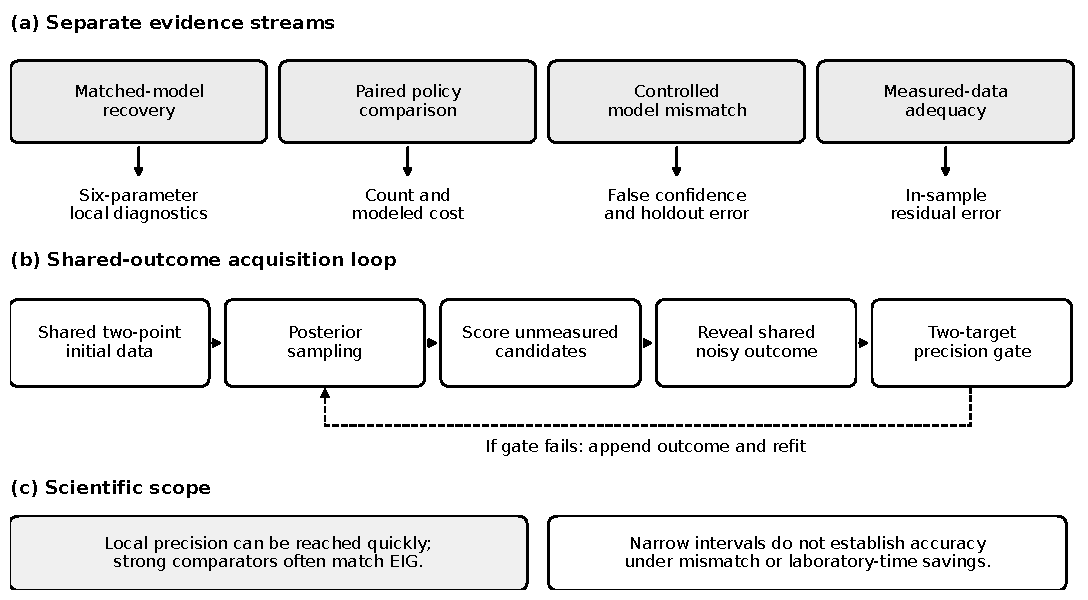
\includegraphics[width=\textwidth,height=0.38\textheight,keepaspectratio]{assets/study-workflow.pdf}
\caption{Study structure separating matched-model recovery,
acquisition-policy comparison, controlled structural mismatch, and
measured-data adequacy.}
\end{figure*}

\hypertarget{research-questions-and-evidence-scope}{%
\section{Research Questions and Evidence
Scope}\label{research-questions-and-evidence-scope}}

The study is organized around six research questions. \emph{RQ1} asks
whether the implemented six-coordinate inference problem is locally
sensitive in all active directions and whether the posterior computation
can recover known matched-model parameters. \emph{RQ2} asks whether
greedy raw EIG reaches one declared local precision gate with fewer
measurements than predictive variance and Laplace D-optimality when
every policy sees identical candidate outcomes. \emph{RQ3} asks the
corresponding question for EIG per prespecified modeled cost. \emph{RQ4}
asks whether the final posterior predicts a disjoint 23-point latent
holdout and recovers all six generating parameters. \emph{RQ5} asks how
well the low-order forward laws describe accepted public measured
records in sample. \emph{RQ6} asks whether the same local precision gate
remains truth-accurate under three fixed structural departures and
whether EIG separates from strong acquisition comparators there.

The evidence ladder shown above prevents answers from being combined
beyond their design. Local Fisher rank is not global identifiability;
matched-model recovery is not validation on real ferrites; posterior
precision is not truth proximity; and in-sample measured residuals are
not held-out predictive accuracy. The acquisition result is therefore an
algorithmic, model-conditional comparison under a finite library and a
local gate. This explicit estimand is narrower than ``optimal
magnetic-component identification,'' but it is reproducible and
falsifiable.

The current frozen evidence contains eight policies: raw EIG, EIG
divided by modeled cost, deterministic and randomized channel-balanced
traversal, predictive variance under raw and per-cost objectives, and
Laplace D-optimality under raw and per-cost objectives. The four direct
strong- comparator contrasts were declared before the confirmatory seed
results were aggregated. The fixed and randomized traversals remain
useful contextual baselines, but they are not evidence that EIG
dominates modern acquisition heuristics.
\href{https://github.com/hoangduong6210/EIG-bayesian-for-Recover-potential-Physical-Parameter-of-MagComponent/blob/927bbcb6d0b862598fae87d2575a872bbd79b5f1/wiki/evidence/Evidence-Sources.md\#e1}{Campaign
source E1}

\hypertarget{related-work}{%
\section{Related Work}\label{related-work}}

\hypertarget{magnetic-loss-and-permeability-models}{%
\subsection{Magnetic loss and permeability
models}\label{magnetic-loss-and-permeability-models}}

The Steinmetz power law remains a compact engineering description for
sinusoidal loss, while loss-separation and hysteresis models provide
more physical
decompositions~\citep{steinmetz1892, bertotti1988, jiles1986}. Converter
waveforms motivated modified and generalized Steinmetz relations that
integrate the instantaneous flux-density trajectory or use waveform
correction factors~\citep{reinert2001, li2001, venkatachalam2002}.
Measurement-led and loss-separation approaches further show why
coefficients fitted under one waveform or operating window need not
transfer unchanged to another ~\citep{vandenbossche2004, roshen2007}.
Subsequent work improved practical loss calculation and reviewed the
physical contributions to loss in soft
ferrites~\citep{muehlethaler2012, dobak2022}. Textbook treatments
emphasize that material law, geometry, winding, and thermal assumptions
must remain distinct in component design
~\citep{snelling1988, mclyman2011}.

Frequency-dispersive permeability is commonly described through
relaxation or resonance spectra. The Cole--Cole law introduced a
broadened relaxation distribution~\citep{cole1941}; applying its
algebraic form to permeability is an engineering adaptation rather than
a claim that ferrite magnetization is a dielectric process. Classical
ferrite dispersion theory and measurements of Mn--Zn and Ni--Zn ferrites
show that domain-wall motion, rotational processes, resonance, and
relaxation can all shape \(\mu'\) and
\(\mu''\)~\citep{snoek1948, tsutaoka2003}. The single-pole model used
here is therefore intentionally diagnostic: a large loss-component
residual is evidence for missing dynamics, not a parameter-estimation
failure alone.

Open magnetic datasets now permit reproducible comparisons beyond
individual vendor plots. MagNet provides systematically measured
core-loss data across materials and excitations~\citep{magnet2022},
while the LEA material database publishes machine-readable permeability
and loss records with source metadata~\citep{materialdatabase}. Public
data improve traceability but do not substitute for a controlled
multi-lot characterization campaign.

\hypertarget{bayesian-calibration-and-experimental-design}{%
\subsection{Bayesian calibration and experimental
design}\label{bayesian-calibration-and-experimental-design}}

Bayesian calibration represents parameter uncertainty conditional on a
forward model, likelihood, and prior~\citep{gelman2013}.
Computer-experiment literature distinguishes emulator uncertainty,
observation error, calibration parameters, and structural
discrepancy~\citep{sacks1989, kennedy2001}. Validation frameworks
consequently compare predictions with observations rather than treating
posterior concentration as proof of physical validity
~\citep{bayarri2007}. Ignoring discrepancy can bias inferred physical
parameters and produce overconfident
extrapolation~\citep{brynjarsdottir2014}. Calibration theory for
imperfect simulators also demonstrates that the physical parameter and
discrepancy can be confounded unless additional structure is
imposed~\citep{tuo2015, plumlee2017}. We do not introduce an
unidentified discrepancy process into the present six-parameter fit;
instead, measured residuals are reported as a separate adequacy
diagnostic.

Bayesian experimental design formalizes the value of a proposed
observation through expected utility. Lindley's information criterion
~\citep{lindley1956}, foundational
reviews~\citep{chaloner1995, ryan2016}, and classical optimum-design
methods~\citep{atkinson2007} motivate the EIG criterion used here.
Estimation remains challenging because the predictive density is
generally unavailable; relevant strategies include Laplace and MCMC
approximations~\citep{ryan2003}, nested Monte Carlo
~\citep{rainforth2018}, multilevel estimators~\citep{goda2020},
stochastic simulation-based optimization ~\citep{huan2013}, and
variational bounds~\citep{foster2019}. Adaptive-policy amortization
offers a scalable direction for longer experimental sequences
~\citep{foster2021}, but the present work deliberately uses a
transparent one-step ranking over a finite candidate library.

Information-based acquisition connects Shannon entropy and
Kullback--Leibler divergence to active data selection
~\citep{shannon1948, kullback1951, mackay1992}. Classical D-optimal
design instead optimizes a determinant of an information matrix and is
linked to equivalence theorems~\citep{kiefer1960, atkinson2007}. These
criteria coincide only under particular approximations; the fixed
traversal used in the reported benchmark is neither of them.

\hypertarget{magnetic-core-models}{%
\section{Magnetic-Core Models}\label{magnetic-core-models}}

\hypertarget{core-loss}{%
\subsection{Core loss}\label{core-loss}}

For sinusoidal excitation within a specified operating window, the
Steinmetz model is
\[P_v(f,B_{\mathrm{pk}})=k f^{\alpha}B_{\mathrm{pk}}^{\beta},
  \label{eq:steinmetz}\] where \(P_v\) is volumetric loss and
\((k,\alpha,\beta)\) are inferred parameters ~\citep{steinmetz1892}. The
units of \(k\) depend on the units used for \(P_v\), \(f\), and
\(B_{\mathrm{pk}}\). The implemented Steinmetz equation is not
temperature dependent in the present implementation. Measured-data
analysis therefore uses a specified temperature subset; the
structural-mismatch experiment separately tests the consequences of
extrapolating this isothermal model across temperature. More general
waveform-dependent loss equations remain important for converter
application studies~\citep{reinert2001, muehlethaler2012}.

\hypertarget{complex-permeability}{%
\subsection{Complex permeability}\label{complex-permeability}}

We adopt the \(e^{j2\pi ft}\) time convention and write
\(\mu_r=\mu'-j\mu''\), so the reported loss component is
\(\mu''=-\operatorname{Im}\mu_r\geq0\) for a passive response. The
relative complex permeability is represented with a single Cole--Cole
relaxation~\citep{cole1941}, \[\mu_r(f)=1+\frac{\mu_s-1}
 {1+\left(jf/f_{\mathrm{rel}}\right)^{1-a_{\mathrm{cc}}}},
 \label{eq:colecole}\] where \(\mu_s\) is low-frequency permeability,
\(f_{\mathrm{rel}}\) is a relaxation frequency, and \(a_{\mathrm{cc}}\)
broadens the relaxation. Storage and loss components are evaluated
separately because a model can fit \(\mu'\) while failing to represent
\(\mu''\). A one-pole model is a deliberate low-order approximation, not
a complete ferrite loss model.

The implemented Cole--Cole equation fixes the high-frequency asymptote
to unity and absorbs the angular-frequency convention into
\(f_{\mathrm{rel}}\). The real and loss components follow from the same
complex denominator, which prevents independent tuning of \(\mu'\) and
\(\mu''\). For an optional inductance channel, the real component is
mapped through \(L_m=\mu_0\mu' N^2A_e/\ell_e\) using specified geometry
~\citep{snelling1988, mclyman2011}. Geometry is never inferred jointly
with material parameters in the present study.

\hypertarget{validity-window}{%
\subsection{Validity window}\label{validity-window}}

Both forward laws are isothermal and evaluated only inside specified
data ranges. A data point is defined by channel, frequency, peak flux
density, and temperature. Core-loss points require positive
\(B_{\mathrm{pk}}\); permeability points use small-signal records. The
likelihood rejects mixed temperature cohorts. Measured permeability uses
material-specific cohorts of \(25\pm0.75\,^{\circ}\mathrm C\) for N87
and \(30\pm0.75\,^{\circ}\mathrm C\) for N95. Measured core loss uses
\(25\pm0.5\,^{\circ}\mathrm C\) for N49, N87, and N95, and
\(100\pm0.5\,^{\circ}\mathrm C\) for 3C95. These restrictions prevent an
apparently precise posterior from silently extrapolating across
temperature, waveform, or excitation regime.

\begin{table*}[t]
\centering
\small
\caption{Physical parameters and active inference
coordinates.}
\setlength{\tabcolsep}{4pt}
\begin{tabular}{@{}
  >{\raggedright\arraybackslash}p{(\textwidth - 8\tabcolsep) * \real{0.20}}
  >{\raggedright\arraybackslash}p{(\textwidth - 8\tabcolsep) * \real{0.20}}
  >{\raggedright\arraybackslash}p{(\textwidth - 8\tabcolsep) * \real{0.20}}
  >{\raggedright\arraybackslash}p{(\textwidth - 8\tabcolsep) * \real{0.20}}
  >{\raggedright\arraybackslash}p{(\textwidth - 8\tabcolsep) * \real{0.20}}@{}}

\toprule
\begin{minipage}[b]{\linewidth}\raggedright
Physical parameter
\end{minipage} & \begin{minipage}[b]{\linewidth}\raggedright
Active coordinate
\end{minipage} & \begin{minipage}[b]{\linewidth}\raggedright
Role
\end{minipage} & \begin{minipage}[b]{\linewidth}\raggedright
Principal response
\end{minipage} & \begin{minipage}[b]{\linewidth}\raggedright
Main limitation
\end{minipage} \\
\midrule

\(k\) & \(\log k\) & core-loss scale & \(P_v\) & units follow the
declared convention \\
\(\alpha\) & \(\alpha\) & frequency exponent & \(P_v\) & local to
sinusoidal, isothermal data \\
\(\beta\) & \(\beta\) & flux-density exponent & \(P_v\) & no waveform or
DC-bias dependence \\
\(\mu_s\) & \(\log\mu_s\) & low-frequency permeability & \(\mu',L_m\) &
fixed rather than inferred geometry \\
\(f_{\mathrm{rel}}\) & \(\log f_{\mathrm{rel}}\) & relaxation frequency
& \(\mu',\mu''\) & one effective relaxation only \\
\(a_{\mathrm{cc}}\) & \(a_{\mathrm{cc}}\) & relaxation broadening &
\(\mu',\mu''\) & no multiple resonances \\
\bottomrule
\end{tabular}
\end{table*}

\hypertarget{bayesian-calibration-and-design}{%
\section{Bayesian Calibration and
Design}\label{bayesian-calibration-and-design}}

Let
\(\theta=(\log k,\alpha,\beta,\log\mu_s,\log f_{\mathrm{rel}}, a_{\mathrm{cc}})\)
denote the active transformed parameters. Log coordinates enforce
positivity of scale parameters while retaining direct coordinates for
the exponents. For observation \(y_o\) at design \(d_o\), the likelihood
is \[p(\mathbf y\mid\theta,\mathbf d)=
 \prod_o \mathcal N\!\left(y_o;F_o(\theta,d_o),\sigma_o^2\right),\] with
fixed relative scales. Synthetic scales are 3\% for core loss, 2\% for
\(\mu'\), 5\% for \(\mu''\), and 1\% for inductance; measured records
use a 3\% relative scale as a weighting model. The posterior is
\[p(\theta\mid\mathbf y,\mathbf d)\propto
 p(\mathbf y\mid\theta,\mathbf d)p(\theta).\] Priors are defined
directly in the transformed space used by the sampler, so no
inverse-transform Jacobian is added to this active-coordinate density.
Bounds encode physically admissible numerical domains, not empirical
proof that the chosen model is correct.

The six coordinates divide into two response blocks in the likelihood
but are sampled jointly. Core-loss observations directly update
\((\log k,\alpha,\beta)\), while permeability and inductance
observations update
\((\log\mu_s,\log f_{\mathrm{rel}},a_{\mathrm{cc}})\). Joint sampling
retains a single posterior contract and permits one acquisition library
to contain all channels; it does not create physical coupling absent
from the forward laws. The parameter table makes this structural
separation explicit.

Four uncertainty sources must be distinguished. \emph{Parameter
uncertainty} is represented by posterior draws conditional on the chosen
model and fixed geometry. \emph{Observation uncertainty} enters through
the declared Gaussian scale. \emph{Monte Carlo uncertainty} arises
because posterior and EIG integrals are approximated by finite samples.
\emph{Structural uncertainty} is exposed by measured residuals but is
not parameterized in the likelihood. Only the first three are quantified
in parts of the present workflow; an EIG score interval is therefore not
a total physical-uncertainty interval.

\hypertarget{posterior-computation-and-diagnostics}{%
\subsection{Posterior computation and
diagnostics}\label{posterior-computation-and-diagnostics}}

Posterior sampling uses the affine-invariant ensemble construction
~\citep{goodman2010} implemented by \texttt{emcee}~\citep{foreman2013}.
Recovery and measured-data fits retain 5000 steps after 1000 warm-up
steps for each of 48 walkers. Matched-model acquisition states use a
stricter adaptive contract: 4000 warm-up steps, at least 20,000 retained
steps, checks every 10,000 additional steps, and a hard ceiling of
80,000 retained steps. The same state-keyed chain is extended rather
than restarted. Initial states are perturbations of the fixed prior
center, never the hidden generating truth. A state is accepted only with
finite integrated autocorrelation estimates, at least 50 retained steps
per autocorrelation time, effective sample size at least 400, mean
acceptance between 0.20 and 0.60, and finite log probability for every
retained sample. Failure at the hard ceiling invalidates that policy
record.

These checks follow the principle of comparing Monte Carlo variation
with between-sequence behavior~\citep{gelman1992} and modern
effective-sample-size practice~\citep{vehtari2021}, but interacting
ensemble walkers are not treated as independent chains. Accordingly, the
paper does not report a conventional \(\widehat R\) for the ensemble.
Diagnostic failure invalidates a measured fit for quantitative
publication rather than being repaired by discarding an unfavorable
seed.

Matched-model recovery also exercises the complete forward--likelihood--
sampler--summary path against known generating values. It is an
implementation check related to posterior-quantile
validation~\citep{cook2006}, but five independent fits do not constitute
simulation-based calibration ~\citep{talts2018}. A calibrated rank
experiment would require many more prior-predictive replications and a
uniform-rank diagnostic. Posterior and residual graphics are interpreted
as part of a Bayesian workflow rather than as substitutes for numerical
diagnostics~\citep{gelman1996, gabry2019}.

The local Fisher approximation~\citep{fisher1922} is
\[\mathcal I_{ij}=\sum_o\frac{1}{\sigma_o^2}
 \frac{\partial F_o}{\partial\theta_i}
 \frac{\partial F_o}{\partial\theta_j}.\] Its spectrum is computed over
the exact active vector and with reported scaling. A large condition
number indicates locally sloppy combinations but does not by itself
establish global non-identifiability~\citep{gutenkunst2007}. Geometric
analyses of sloppy models likewise interpret broad eigenvalue spectra as
anisotropic distinguishability, not as a universal parameter
ranking~\citep{transtrum2015}. The spectrum is therefore reported
together with its dimension and scaling convention.

Let \(\mathcal D_t=(\mathbf y_t,\mathbf d_t)\) denote the observations
available before acquisition step \(t\). For candidate \(d\), the
one-step EIG is the conditional mutual
information~\citep{lindley1956, chaloner1995} \[\mathrm{EIG}_t(d)=
 \mathbb E_{\substack{\theta\sim p(\theta\mid\mathcal D_t)\\
 y\sim p(y\mid\theta,d)}}
 \left[
 \log p(y\mid\theta,d)-\log p(y\mid d,\mathcal D_t)
 \right],
 \label{eq:eig}\] where \[p(y\mid d,\mathcal D_t)=
 \int p(y\mid\vartheta,d)
 p(\vartheta\mid\mathcal D_t)\,d\vartheta .\] For outer draws
\((\theta_i,y_i)\) and inner posterior draws \(\vartheta_{ij}\), the
implemented nested estimator is \[\begin{aligned}
 \widehat U(d)=\frac{1}{N}\sum_{i=1}^{N}\bigg[&
 \log p(y_i\mid\theta_i,d)\\[-0.2ex]
 &-\log\!\left\{\frac{1}{M}\sum_{j=1}^{M}
 p(y_i\mid\vartheta_{ij},d)\right\}\bigg].
 \end{aligned}
 \label{eq:nmc}\] Finite inner budgets introduce bias through the
logarithm and finite outer budgets introduce variance; close candidates
can therefore exchange rank ~\citep{rainforth2018, goda2020}. The
convergence campaign described below tests ranking and downstream
endpoint stability rather than assuming one budget is sufficient.

The reported estimator draws outer parameter--observation pairs and uses
inner posterior draws to approximate the posterior-predictive
density~\citep{ryan2003, rainforth2018}. Each score is repeated 40
times; the mean, standard error, 95\% Monte Carlo interval, and top-rank
frequency are retained. Candidate streams are seeded from a stable key
comprising channel, frequency, flux density, and temperature, so list
permutation cannot change a design's draws. We evaluate two distinct
objectives: raw EIG for the measurement-count endpoint and EIG divided
by a prespecified modeled acquisition cost for the total-cost endpoint.
These intervals quantify repeated nested-Monte-Carlo variability
conditional on the retained posterior draws and model; they exclude
chain-to-chain, structural-model, geometry, and noise-model uncertainty.

\hypertarget{paired-sequential-policy}{%
\subsection{Paired sequential policy}\label{paired-sequential-policy}}

After the same two initial observations---\(P_v\) at 30 kHz, 0.05 T, and
\(25\,^{\circ}\mathrm C\), and \(\mu'\) at 10 kHz and
\(25\,^{\circ}\mathrm C\)---each policy selects one unrevealed
candidate, receives its pre-generated noisy outcome, refits the
posterior, and checks the common precision gate. The registry contains
exactly eight policies. Raw EIG and predictive variance maximize their
unscaled criteria; their per-cost forms divide those criteria by the
declared channel cost. Laplace D-optimality greedily maximizes the
log-determinant increment of a local posterior-precision approximation,
with an analogous per-cost form. The contextual comparators are
deterministic fixed and seeded randomized channel-balanced traversals.
The fixed traversal is not called a uniform grid, and neither traversal
is a space-filling or globally optimal design. All policies share the
candidate library, latent truth, candidate-indexed noisy outcomes,
maximum budget, and stopping rule. The candidate library is isothermal,
so it contains no temperature-only duplicates of the implemented forward
laws. The numerical settings are summarized below.

For clarity, predictive variance is noise-normalized, not an unscaled
comparison of responses with different physical units. With posterior
response draws \(F_d(\theta)\), its score is \[U_{\mathrm{PV}}(d)=
 \frac{\operatorname{Var}[F_d(\theta)\mid\mathcal D_t]}{\sigma_d^2}.\]
The denominator uses the declared channel noise fraction times the
median absolute posterior prediction, with the implementation's
\(10^{-9}\) numerical floor. Irreducible observation variance is not
added to the numerator. For posterior covariance \(\Sigma\) in active
coordinates and response gradient \(g_d\) at the posterior-mean
coordinate vector, the Laplace score is \[U_{\mathrm L}(d)=\tfrac12\log
 \left(1+\frac{g_d^{\mathsf T}\Sigma g_d}{\sigma_d^2}\right).\] It uses
central finite differences with relative step \(10^{-5}\) and the same
noise convention. This is a local Gaussian information approximation
rather than a full nonlinear Fisher-greedy policy. In the
linear-Gaussian limit, the raw Laplace score is a monotone function of
noise-normalized predictive variance, explaining why their rankings can
agree. Dividing the two scores by varying channel costs need not
preserve this agreement.

The stopping statistic is the half-width of the central 90\% posterior
interval for the noise-free latent mean response divided by the absolute
posterior median. Observation noise is not added to this gate. The two
fixed targets are
\(P_v(100\,\mathrm{kHz},0.1\,\mathrm T,25\,^{\circ}\mathrm C)\) at 8\%
and \(L_m(100\,\mathrm{kHz},25\,^{\circ}\mathrm C)\) at 5\%. This is a
local precision criterion: it checks neither truth proximity,
six-parameter recovery, other channels, held-out performance, nor model
adequacy. A policy that misses either threshold is recorded as a failure
at the maximum budget. Candidate EIG integrates over the joint
six-parameter posterior; only the stopping and evaluation endpoint is
restricted to these two responses.

\begin{table*}[t]
\centering
\small
\caption{Isothermal acquisition library, observation scales, and modeled
costs.}
\setlength{\tabcolsep}{4pt}
\begin{tabular}{@{}
  >{\raggedright\arraybackslash}p{(\textwidth - 10\tabcolsep) * \real{0.12}}
  >{\raggedright\arraybackslash}p{(\textwidth - 10\tabcolsep) * \real{0.29}}
  >{\raggedright\arraybackslash}p{(\textwidth - 10\tabcolsep) * \real{0.17}}
  >{\raggedright\arraybackslash}p{(\textwidth - 10\tabcolsep) * \real{0.10}}
  >{\raggedright\arraybackslash}p{(\textwidth - 10\tabcolsep) * \real{0.16}}
  >{\raggedright\arraybackslash}p{(\textwidth - 10\tabcolsep) * \real{0.16}}@{}}

\toprule
\begin{minipage}[b]{\linewidth}\raggedright
Channel
\end{minipage} & \begin{minipage}[b]{\linewidth}\raggedright
Frequencies (kHz)
\end{minipage} & \begin{minipage}[b]{\linewidth}\raggedright
\(B_{\mathrm{pk}}\) (T)
\end{minipage} & \begin{minipage}[b]{\linewidth}\raggedright
Points
\end{minipage} & \begin{minipage}[b]{\linewidth}\raggedright
Relative noise
\end{minipage} & \begin{minipage}[b]{\linewidth}\raggedright
Modeled cost
\end{minipage} \\
\midrule

\(P_v\) & 30, 50, 100, 200, 300, 500 & 0.05, 0.10, 0.20 & 18 & 3\% &
60 \\
\(\mu'\) & 10, 30, 100, 300, 500, 1000, 2000, 3000 & 0 & 8 & 2\% & 20 \\
\(\mu''\) & 10, 30, 100, 300, 500, 1000, 2000, 3000 & 0 & 8 & 5\% &
20 \\
\(L_m\) & 10, 100, 1000 & 0 & 3 & 1\% & 15 \\
\bottomrule
\end{tabular}
\end{table*}

All 37 candidates are at \(25\,^{\circ}\mathrm C\). Modeled costs are
positive prespecified units used for the modeled-cost objective and
endpoint; they are not measured instrument or laboratory durations. The
two initial observations belong to the same library and count toward the
stopping total.

\hypertarget{computational-reproducibility}{%
\section{Computational
Reproducibility}\label{computational-reproducibility}}

All experiments use fixed software versions, specified model and
inference settings, explicit data selections, and deterministic random
seeds. Results are retained at the individual-seed level and are
accepted for aggregation only when all prespecified validity gates pass.

\hypertarget{tab:protocol}{}
\begin{table*}[t]
\centering
\small
\caption{Computational settings for the matched-model acquisition
experiment. The structural-mismatch sampler is specified separately
below.}
\setlength{\tabcolsep}{4pt}
\begin{tabular}{@{}
  >{\raggedright\arraybackslash}p{(\textwidth - 2\tabcolsep) * \real{0.30}}
  >{\raggedright\arraybackslash}p{(\textwidth - 2\tabcolsep) * \real{0.70}}@{}}

\toprule
\begin{minipage}[b]{\linewidth}\raggedright
Item
\end{minipage} & \begin{minipage}[b]{\linewidth}\raggedright
Setting
\end{minipage} \\
\midrule

Ensemble sampler & 48 walkers; acquisition chains retain 20,000--80,000
adaptively \\
Convergence criteria & ESS \(\geq400\); steps/\(\tau\geq50\) \\
Acceptance criterion & \(0.20\)--\(0.60\) \\
Nested EIG & 1200 outer; 400 inner; 40 score replicates \\
Sequential budget & at most 25 measurements \\
Acquisition endpoints & raw EIG/count; EIG/cost/modeled cost \\
Temperature cohorts & material and channel specific, as stated in
text \\
Precision gate & latent mean response: 8\% \(P_v\); 5\% \(L_m\) \\
\bottomrule
\end{tabular}
\end{table*}

The analysis checks all required seed and material cases before forming
aggregate summaries. Records with nonfinite values, failed convergence,
or boundary-active parameters are excluded according to criteria
specified before evaluation. Numerical statements, tables, and figures
are generated programmatically from the same complete set of accepted
records, avoiding manual transcription or selective replacement of
outcomes.

\hypertarget{estimator-budget-qualification}{%
\subsection{Estimator-budget
qualification}\label{estimator-budget-qualification}}

The nested estimator was qualified before the 30-seed acquisition
campaign. Twelve posterior states were formed from four seeds
(7100--7103) after 2, 4, and 6 observations. At each state, 27 candidate
settings crossed outer budgets \(\{100,300,900\}\), inner budgets
\(\{50,100,300\}\), and replicate counts \(\{5,10,20\}\). Every setting
was compared with a 1200-outer, 400-inner, 40-replicate reference. Two
sentinel states were additionally recomputed at 2400 outer and 800 inner
draws with 40 replicates. Prefix-nested random streams made the
lower-budget samples literal prefixes of the larger calculations,
reducing irrelevant differences between settings.

The acceptance decision combined the stable top candidate, Spearman rank
correlation, score-interval overlap, relative reference regret, and
exact agreement of downstream count and modeled-cost endpoints. Ten
disjoint seeds (7200--7209) supplied that downstream check. The selected
setting was then locked before the confirmatory acquisition seeds
7300--7329 were evaluated. This separation prevents selecting an
estimator budget because it happened to produce the most favorable
headline comparison.

\begin{table*}[t]
\centering
\small
\caption{Evidence layers of the matched-model and measured-data
evaluation.}
\setlength{\tabcolsep}{4pt}
\begin{tabular}{@{}
  >{\raggedright\arraybackslash}p{(\textwidth - 6\tabcolsep) * \real{0.20}}
  >{\raggedright\arraybackslash}p{(\textwidth - 6\tabcolsep) * \real{0.26}}
  >{\raggedright\arraybackslash}p{(\textwidth - 6\tabcolsep) * \real{0.33}}
  >{\raggedright\arraybackslash}p{(\textwidth - 6\tabcolsep) * \real{0.21}}@{}}

\toprule
\begin{minipage}[b]{\linewidth}\raggedright
Layer
\end{minipage} & \begin{minipage}[b]{\linewidth}\raggedright
Prespecified cases
\end{minipage} & \begin{minipage}[b]{\linewidth}\raggedright
Retained public evidence
\end{minipage} & \begin{minipage}[b]{\linewidth}\raggedright
Scientific role
\end{minipage} \\
\midrule

Matched recovery & 5 generating seeds & seed-level parameter summaries &
implementation check \\
Estimator states & \(4\times3=12\) & state records and flattened
posterior samples & budget qualification \\
Estimator grid & 27 budget combinations across 12 states & 108
candidate-score records plus 12 references & ranking stability \\
Doubled-budget audit & 2 sentinel states & 2 doubled-budget score
records & reference sensitivity \\
Downstream validation & 10 seeds & 10 policy endpoint records & endpoint
stability \\
Confirmatory acquisition & 30 paired seeds & 30 complete policy
trajectories & count and cost endpoints \\
Measured adequacy & declared material/source pairs & aggregate metrics
and disclosed exclusions & model discrepancy diagnostic \\
\bottomrule
\end{tabular}
\end{table*}

The public audit projection retains the campaign records needed to
reconstruct the acquisition endpoints and estimator decision while
removing machine paths and scheduler metadata. Posterior arrays are
retained flattened over sampling draws; because walker and iteration
indices are not present, they are not described as raw MCMC chains. The
compact frozen summary authenticates the reported measured-fit
aggregates and exclusions, but the audit projection does not
independently reconstruct those fits. Raw upstream measured curves
remain governed by their source repositories and are not redistributed
here.

\hypertarget{evaluation-protocol}{%
\section{Evaluation Protocol}\label{evaluation-protocol}}

Five fixed seeds are used for matched-model recovery. A disjoint,
prespecified set of seeds is used for the paired acquisition comparison
only after the nested-Monte-Carlo setting passes a separate convergence
study. That study uses prefix-nested common random numbers and a
deterministic paired bootstrap of the replicate-mean selector; it
requires stable candidate and reference winners, rank correlation,
score-interval overlap, low reference regret, and downstream endpoint
agreement. The policies share initial observations, candidate library,
realized candidate outcomes, noise policy, budget, and stopping rule.
Results include per-seed counts, modeled costs, and failures, not only
an aggregate ratio. The stopping rule concerns posterior precision of
two latent mean responses and is not an accuracy or coverage guarantee.

For recovery, observations are generated from the same six-parameter
forward family used in inference. A parameter vector is drawn
independently for each seed from a datasheet prior fixed before that
draw; the prior is never rebuilt from the realized truth. Sampler
walkers are initialized around the fixed prior center, not around the
hidden generating vector. Observation noise is then generated
independently. This is a prior-predictive matched-model design: it
removes oracle centering while retaining favorable equality between the
data-generating and inference model families. The reported error is the
absolute relative difference between posterior median and the generating
value. The interval statistic counts whether that value falls within the
equal-tailed 90\% model-conditional posterior credible interval. With
only five seeds, the count is a descriptive implementation check, not a
coverage experiment. The Fisher matrix is evaluated in the exact
transformed coordinate system used by sampling.

For the paired acquisition analysis, a stable design-keyed seed
generates one noisy observation for every candidate before any policy is
run. A policy reveals the already generated value when it selects that
design. Thus policy order cannot change the noise attached to a
candidate, and all policies in a seed share the same latent truth and
candidate outcome map. The 30 paired differences are the unit of
analysis. Descriptive means, medians, standard deviations, win and
failure rates, and percentile intervals are computed from those
differences. The reported confidence interval uses 10,000 deterministic
paired bootstrap resamples. It quantifies between-seed variation in this
matched-model experiment and is not a population-wide material claim.

The measured evaluation uses public complex-permeability curves for
specified N95, N87, and 3C95 source/material pairs and datasheet
core-loss curves for N49, N87, N95, and 3C95~\citep{materialdatabase}.
Input-data versions, temperature cohorts, unit conversions, and range
filters were fixed before inference. Storage/loss permeability errors,
core-loss residuals, boundary activity, and operating-window coverage
are reported separately. Records with failed convergence or active
boundary flags are retained for diagnostic review but excluded from
aggregate numerical claims.

Core-loss adequacy is summarized by in-sample relative root-mean-square
error (RRMSE) within each temperature cohort. Permeability adequacy is
evaluated separately for storage and loss components because combining
them can conceal a poor \(\mu''\) fit behind the larger magnitude of
\(\mu'\). These metrics assess the selected low-order model on observed
records; they are neither held-out prediction errors nor component-level
thermal validation.

\hypertarget{controlled-structural-mismatch-experiment}{%
\subsection{Controlled structural-mismatch
experiment}\label{controlled-structural-mismatch-experiment}}

The separate MM-3 experiment holds the inference family fixed while
changing the data generator. Thirty independent prior-predictive seeds,
10100--10129, are crossed with four prespecified scenarios. Within each
of the resulting 120 tasks, all eight policies share the generating
parameter vector and the candidate-indexed noisy outcomes. The scenarios
are a matched control, two-pole permeability, temperature/curvature core
loss, and a combined departure. These are controlled perturbations, not
fits of a discrepancy law to the measured residuals. The combined case
has its own larger coefficients; it is not simply the sum of the two
single-departure cases.

For the loss generator, define \(x=\log_{10}(f/100\,\mathrm{kHz})\) and
\(z=\log_{10}(B_{\mathrm{pk}}/0.1\,\mathrm T)\). The generated latent
loss is \[P_v^{\star}=k f^\alpha B_{\mathrm{pk}}^\beta
 \exp\{s_T(T-25)+c_f x^2+c_{fB}xz\}.\] Here \(T\) is the numerical
temperature in degrees Celsius and \(s_T\) has units of inverse degrees
Celsius. The two-pole permeability generator is
\[\mu_r^{\star}(f)=1+(\mu_s-1)
 \sum_{r=1}^{2}\frac{w_r}
 {1+[jf/(m_r f_{\mathrm{rel}})]^{1-\widetilde a_r}},\] where
\(w_1=1-w_2\) and
\(\widetilde a_r=\min\{0.95,\max[0,a_{\mathrm{cc}}+\delta_r]\}\). The
inductance generator uses the real part of this permeability and the
same fixed geometry as inference. The registered coefficients are shown
below; none is inferred by the six-parameter posterior.

\begin{table*}[t]
\centering
\small
\caption{Fixed structural-departure coefficients in the data
generator.}
\setlength{\tabcolsep}{4pt}
\begin{tabular}{@{}
  >{\raggedright\arraybackslash}p{(\textwidth - 12\tabcolsep) * \real{0.24}}
  >{\raggedright\arraybackslash}p{(\textwidth - 12\tabcolsep) * \real{0.08}}
  >{\raggedright\arraybackslash}p{(\textwidth - 12\tabcolsep) * \real{0.15}}
  >{\raggedright\arraybackslash}p{(\textwidth - 12\tabcolsep) * \real{0.17}}
  >{\raggedright\arraybackslash}p{(\textwidth - 12\tabcolsep) * \real{0.12}}
  >{\raggedright\arraybackslash}p{(\textwidth - 12\tabcolsep) * \real{0.12}}
  >{\raggedright\arraybackslash}p{(\textwidth - 12\tabcolsep) * \real{0.12}}@{}}

\toprule
\begin{minipage}[b]{\linewidth}\raggedright
Scenario
\end{minipage} & \begin{minipage}[b]{\linewidth}\raggedright
\(w_2\)
\end{minipage} & \begin{minipage}[b]{\linewidth}\raggedright
\(m_1,m_2\)
\end{minipage} & \begin{minipage}[b]{\linewidth}\raggedright
\(\delta_1,\delta_2\)
\end{minipage} & \begin{minipage}[b]{\linewidth}\raggedright
\(s_T\)
\end{minipage} & \begin{minipage}[b]{\linewidth}\raggedright
\(c_f\)
\end{minipage} & \begin{minipage}[b]{\linewidth}\raggedright
\(c_{fB}\)
\end{minipage} \\
\midrule

Matched control & 0 & 1, 1 & 0, 0 & 0 & 0 & 0 \\
Two-pole permeability & 0.25 & 0.75, 5 & -0.05, 0.18 & 0 & 0 & 0 \\
Temperature/curvature & 0 & 1, 1 & 0, 0 & 0.0035 & 0.08 & 0.05 \\
Combined mismatch & 0.35 & 0.55, 7 & -0.10, 0.25 & 0.0055 & 0.14 &
0.10 \\
\bottomrule
\end{tabular}
\end{table*}

Acquisition retains exactly the 37 unique \(25\,^{\circ}\mathrm C\)
candidates and the original two-target precision gate. Temperatures of
60 and \(100\,^{\circ}\mathrm C\) occur only in the disjoint latent
holdout: replicating temperature-only candidates would add duplicate
information under the isothermal inference model. The mismatch holdout
contains 39 points, extending the matched-model 23-point set by
repeating its eight core-loss points at those two additional
temperatures. Holdout truths are never used for acquisition or stopping.
Thus the cross-temperature result measures extrapolation failure, not
learning from temperature measurements.

Production sampling uses an 80\% differential-evolution and 20\% snooker
move mixture in \texttt{emcee} 3.1.6 with 48 walkers, initialized at
perturbations of the fixed prior center. The differential-evolution
scale is \(2.38/\sqrt{12}\); the snooker scale is 1.7. Each state
discards 80,000 warm-up steps and is checked every 20,000 retained steps
up to a hard limit of 800,000. Every coordinate must have ESS at least
400 and retained length divided by autocorrelation time at least 50,
with finite log probability throughout and mean acceptance in
\([0.05,0.80]\). Two successive checkpoint changes in every
autocorrelation estimate must be no greater than 10\%, measured relative
to the current estimate; hence acceptance cannot occur before 60,000
retained steps. This contract was qualified on two locked
sparse-observation states using independent ensembles without
acquisition endpoints, then fixed before the new seed campaign. Earlier
incomplete campaigns are not pooled with MM-3.

A false-confident outcome is defined before evaluation as reaching the
local width gate while the posterior-median absolute relative error
exceeds 8\% at the core-loss target or 5\% at the inductance target.
Latent-holdout RRMSE and 90\% interval inclusion are reported separately
by channel and temperature. The unit for paired inference remains the
complete seed, and all bootstrap intervals are descriptive, without
multiplicity adjustment. A 90\% interval's inclusion frequency over this
fixed holdout is not a parameter-rank calibration diagnostic. Complete
admission requires all 120 expected tasks and all their policy records
to satisfy the locked validity checks; a partial matrix is not an
alternative confirmatory result.
\href{https://github.com/hoangduong6210/EIG-bayesian-for-Recover-potential-Physical-Parameter-of-MagComponent/blob/927bbcb6d0b862598fae87d2575a872bbd79b5f1/wiki/evidence/Evidence-Sources.md\#e16}{Protocol
and result source E16}

\hypertarget{results}{%
\section{Results}\label{results}}

\hypertarget{identifiability-and-synthetic-recovery}{%
\subsection{Identifiability and synthetic
recovery}\label{identifiability-and-synthetic-recovery}}

The synthetic \(6\times6\) Fisher matrix was full rank. Its eigenvalues
span \(1.24\times10^2\) to \(2.91\times10^6\), giving a condition number
of \(2.35\times10^4\). This broad spectrum indicates strong local
sensitivity anisotropy in the active transformed coordinates; it does
not establish global identifiability. Across five prior-predictive
matched-model data sets, the per-parameter median absolute relative
errors ranged from 0.27\% to 5.85\%. The known values fell within 28 of
30 equal-tailed 90\% model-conditional posterior credible intervals.
This observed inclusion count is descriptive, not a coverage estimate.
\href{https://github.com/hoangduong6210/EIG-bayesian-for-Recover-potential-Physical-Parameter-of-MagComponent/blob/927bbcb6d0b862598fae87d2575a872bbd79b5f1/wiki/evidence/Evidence-Sources.md\#e2}{Result
source E2}

\begin{table*}[t]
\centering
\small
\caption{Five-seed matched-model parameter recovery; errors are absolute
relative errors.}
\setlength{\tabcolsep}{4pt}
\begin{tabular}{@{}
  >{\raggedright\arraybackslash}p{(\textwidth - 8\tabcolsep) * \real{0.20}}
  >{\raggedright\arraybackslash}p{(\textwidth - 8\tabcolsep) * \real{0.20}}
  >{\raggedright\arraybackslash}p{(\textwidth - 8\tabcolsep) * \real{0.20}}
  >{\raggedright\arraybackslash}p{(\textwidth - 8\tabcolsep) * \real{0.20}}
  >{\raggedright\arraybackslash}p{(\textwidth - 8\tabcolsep) * \real{0.20}}@{}}

\toprule
\begin{minipage}[b]{\linewidth}\raggedright
Parameter
\end{minipage} & \begin{minipage}[b]{\linewidth}\raggedright
Mean error
\end{minipage} & \begin{minipage}[b]{\linewidth}\raggedright
Median error
\end{minipage} & \begin{minipage}[b]{\linewidth}\raggedright
SD
\end{minipage} & \begin{minipage}[b]{\linewidth}\raggedright
Truth in 90\% CI
\end{minipage} \\
\midrule

\(k\) & 7.36\% & 5.85\% & 5.94\% & 4/5 \\
\(\alpha\) & 0.40\% & 0.27\% & 0.36\% & 4/5 \\
\(\beta\) & 0.38\% & 0.36\% & 0.25\% & 5/5 \\
\(\mu_s\) & 0.35\% & 0.38\% & 0.17\% & 5/5 \\
\(f_{\mathrm{rel}}\) & 0.91\% & 0.87\% & 0.55\% & 5/5 \\
\(a_{\mathrm{cc}}\) & 0.91\% & 0.62\% & 0.79\% & 5/5 \\
\bottomrule
\end{tabular}
\end{table*}

\href{https://github.com/hoangduong6210/EIG-bayesian-for-Recover-potential-Physical-Parameter-of-MagComponent/blob/927bbcb6d0b862598fae87d2575a872bbd79b5f1/wiki/evidence/Evidence-Sources.md\#e2}{Table
source E2}

\begin{figure*}[t]
\centering
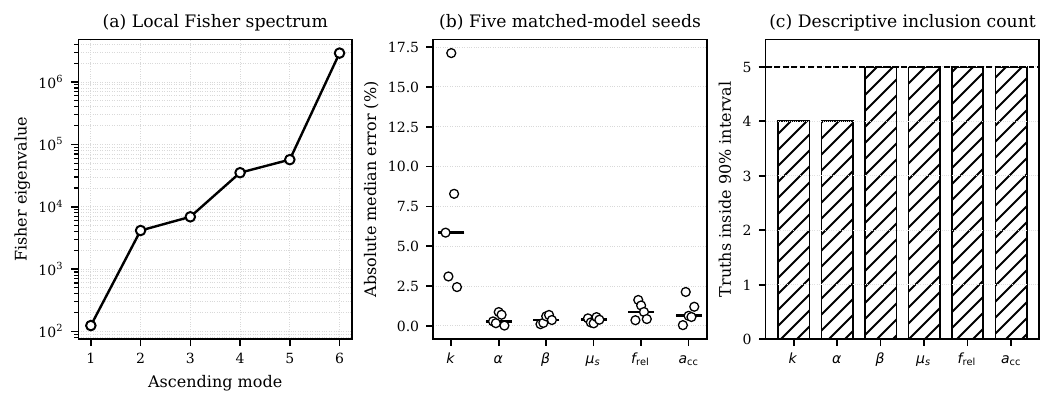
\includegraphics[width=\textwidth,height=0.38\textheight,keepaspectratio]{assets/synthetic-diagnostics.png}
\caption{Local Fisher spectrum and five-seed matched-model recovery.}
\end{figure*}

\hypertarget{nested-estimator-qualification}{%
\subsection{Nested-estimator
qualification}\label{nested-estimator-qualification}}

The conservative reference setting of 1200 outer draws, 400 inner draws,
and 40 score replicates was selected by the prespecified convergence
decision. Against doubled-budget sentinels, minimum top-selector
agreement was 0.9983 for raw EIG and 1.0000 for EIG/cost; minimum
Spearman correlation was 0.9983 and 0.9992, respectively, minimum
score-interval overlap was 0.8710, and maximum relative regret was zero.
Ten downstream validation seeds reproduced the reference count and
modeled-cost endpoints. This qualifies the numerical setting for the
campaign; it does not make each finite EIG score exact or incorporate
structural-model uncertainty.
\href{https://github.com/hoangduong6210/EIG-bayesian-for-Recover-potential-Physical-Parameter-of-MagComponent/blob/927bbcb6d0b862598fae87d2575a872bbd79b5f1/wiki/evidence/Evidence-Sources.md\#e3}{Result
source E3}

\hypertarget{paired-synthetic-acquisition}{%
\subsection{Paired synthetic
acquisition}\label{paired-synthetic-acquisition}}

Raw EIG reached the two-target precision gate in exactly five
measurements, while the deterministic fixed channel-balanced traversal
required nine in all 30 paired seeds. The four-measurement difference
had zero sample variation and a bootstrap 95\% interval of 4.00--4.00
measurements. This 44.4\% reduction is a valid comparison with that
specified baseline, but the strong-comparator results materially narrow
its interpretation.
\href{https://github.com/hoangduong6210/EIG-bayesian-for-Recover-potential-Physical-Parameter-of-MagComponent/blob/927bbcb6d0b862598fae87d2575a872bbd79b5f1/wiki/evidence/Evidence-Sources.md\#e4}{Result
source E4}

\begin{table*}[t]
\centering
\small
\caption{Direct strong-comparator contrasts over 30 paired matched-model
seeds. W/T/L denotes EIG wins, ties, and losses.}
\setlength{\tabcolsep}{4pt}
\begin{tabular}{@{}
  >{\raggedright\arraybackslash}p{(\textwidth - 8\tabcolsep) * \real{0.20}}
  >{\raggedright\arraybackslash}p{(\textwidth - 8\tabcolsep) * \real{0.20}}
  >{\raggedright\arraybackslash}p{(\textwidth - 8\tabcolsep) * \real{0.20}}
  >{\raggedright\arraybackslash}p{(\textwidth - 8\tabcolsep) * \real{0.20}}
  >{\raggedright\arraybackslash}p{(\textwidth - 8\tabcolsep) * \real{0.20}}@{}}

\toprule
\begin{minipage}[b]{\linewidth}\raggedright
Preregistered direct contrast
\end{minipage} & \begin{minipage}[b]{\linewidth}\raggedright
Endpoint
\end{minipage} & \begin{minipage}[b]{\linewidth}\raggedright
Mean difference, comparator \(-\) EIG
\end{minipage} & \begin{minipage}[b]{\linewidth}\raggedright
Bootstrap 95\% CI
\end{minipage} & \begin{minipage}[b]{\linewidth}\raggedright
EIG W/T/L
\end{minipage} \\
\midrule

Raw EIG vs predictive variance & measurement count & 0.00 & {[}0.00,
0.00{]} & 0/30/0 \\
Raw EIG vs Laplace D-optimality & measurement count & 0.00 & {[}0.00,
0.00{]} & 0/30/0 \\
EIG/cost vs predictive variance/cost & modeled cost & -15.17 &
{[}-15.50, -15.00{]} & 0/0/30 \\
EIG/cost vs Laplace D-optimality/cost & modeled cost & 0.00 & {[}0.00,
0.00{]} & 0/30/0 \\
\bottomrule
\end{tabular}
\end{table*}

\href{https://github.com/hoangduong6210/EIG-bayesian-for-Recover-potential-Physical-Parameter-of-MagComponent/blob/927bbcb6d0b862598fae87d2575a872bbd79b5f1/wiki/evidence/Evidence-Sources.md\#e4}{Table
source E4}

All eight policies reached the gate in all 30 seeds. Thus the experiment
gives no evidence that raw EIG outperforms predictive variance or
Laplace D-optimality on measurement count. Under the cost objective,
predictive variance reached the gate at modeled cost 175 in every seed,
whereas EIG/cost used 190 in 29 seeds and 195 once. The cost constants
are prespecified model inputs, not measured laboratory durations.
\href{https://github.com/hoangduong6210/EIG-bayesian-for-Recover-potential-Physical-Parameter-of-MagComponent/blob/927bbcb6d0b862598fae87d2575a872bbd79b5f1/wiki/evidence/Evidence-Sources.md\#e4}{Result
source E4}

\hypertarget{descriptive-selection-path-diagnostic}{%
\subsubsection{Descriptive selection-path
diagnostic}\label{descriptive-selection-path-diagnostic}}

A post hoc diagnostic helps locate why the strong comparators tied or
beat EIG on this gate. On posterior states with identical hashes and
candidate universes, raw EIG and raw predictive variance had mean
Spearman score-rank correlation 0.9967 over 57 states; their final
selected sets had mean Jaccard overlap 0.933, although the complete
ordered path matched in only 11 of 30 seeds. Raw EIG and raw Laplace
D-optimality similarly had mean rank correlation 0.9947 over 36
comparable states and mean selected-set Jaccard overlap 0.867. The raw
utilities therefore placed nearly the same candidates near the top and
usually acquired the same set in a different order, leaving no
measurement-count separation at the common gate.

The cost-normalized comparison diverged at the third acquisition.
EIG/cost selected \(L_m(10\,\mathrm{kHz})\) in 28 of 30 seeds, whereas
predictive variance/cost selected
\(P_v(500\,\mathrm{kHz},0.2\,\mathrm T)\) in 29 of 30. The mean
reduction in the normalized maximum gate ratio was 0.0048 for EIG/cost
and 2.6174 for predictive variance/cost; zero and 30 seeds,
respectively, crossed the gate after that acquisition. This pattern
supports objective--gate misalignment in the present matched-model
benchmark: joint parameter information favored an inductance measurement
while the remaining stopping uncertainty was primarily at the core-loss
target. Because this diagnostic was defined after the comparator result
and uses realized policy paths, it does not establish a general causal
advantage for predictive variance.
\href{https://github.com/hoangduong6210/EIG-bayesian-for-Recover-potential-Physical-Parameter-of-MagComponent/blob/927bbcb6d0b862598fae87d2575a872bbd79b5f1/wiki/evidence/Evidence-Sources.md\#e9}{Diagnostic
source E9}

\begin{figure*}[t]
\centering
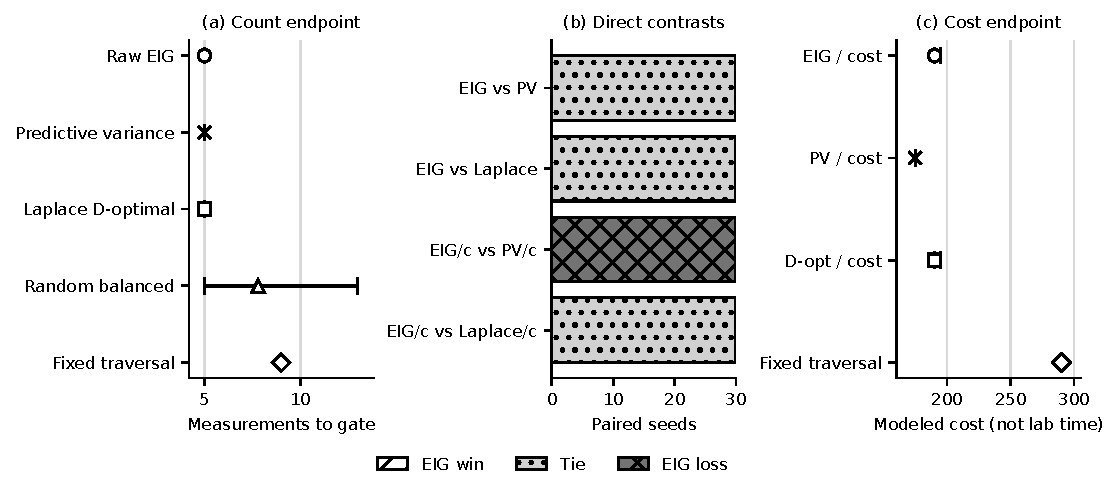
\includegraphics[width=\textwidth,height=0.38\textheight,keepaspectratio]{assets/acquisition-diagnostics.pdf}
\caption{Eight-policy paired acquisition results and four direct
strong-comparator contrasts.}
\end{figure*}

\hypertarget{disjoint-holdout-and-six-parameter-endpoints}{%
\subsection{Disjoint holdout and six-parameter
endpoints}\label{disjoint-holdout-and-six-parameter-endpoints}}

The 23-point latent holdout was excluded from acquisition, policy
selection, and stopping. For raw EIG, mean RRMSE was 3.12\% for core
loss, 1.32\% for \(\mu'\), 3.93\% for \(\mu''\), and 1.20\% for \(L_m\);
mean 90\% latent-interval coverage was 85.8\%, 93.9\%, 90.0\%, and
92.2\%, respectively. EIG/cost gave mean RRMSE 3.15\%, 0.95\%, 2.78\%,
and 0.85\%, with coverage 85.0\%, 93.3\%, 89.4\%, and 93.3\%. These
secondary endpoints do not rescue an acquisition-superiority claim:
predictive-variance and Laplace policies had comparable holdout
performance, while the fixed and randomized traversals were often worse.
\href{https://github.com/hoangduong6210/EIG-bayesian-for-Recover-potential-Physical-Parameter-of-MagComponent/blob/927bbcb6d0b862598fae87d2575a872bbd79b5f1/wiki/evidence/Evidence-Sources.md\#e6}{Result
source E6}

Final 90\% parameter intervals contained a mean 5.13 of six generating
parameters for both EIG objectives. Across policies, however, mean
absolute error for \(k\) remained approximately 25.1\%--30.7\%.
Posterior interval inclusion must therefore not be described as
uniformly precise global six-parameter recovery.
\href{https://github.com/hoangduong6210/EIG-bayesian-for-Recover-potential-Physical-Parameter-of-MagComponent/blob/927bbcb6d0b862598fae87d2575a872bbd79b5f1/wiki/evidence/Evidence-Sources.md\#e6}{Result
source E6}

\hypertarget{preregistered-model-mismatch-campaign}{%
\subsection{Preregistered model-mismatch
campaign}\label{preregistered-model-mismatch-campaign}}

MM-3 evaluated the matched control and three fixed structural departures
over 30 new paired seeds. All 120 scenario--seed tasks passed the
registered sampler contract, all eight policies reached the local
precision gate in every scenario, and the complete sanitized record set
reconstructed the aggregate. This is a synthetic robustness experiment
with latent truth, not a measured- material validation.
\href{https://github.com/hoangduong6210/EIG-bayesian-for-Recover-potential-Physical-Parameter-of-MagComponent/blob/927bbcb6d0b862598fae87d2575a872bbd79b5f1/wiki/evidence/Evidence-Sources.md\#e16}{Result
source E16}

\begin{table*}[t]
\centering
\small
\caption{Raw EIG under the four registered data generators, with 30
paired seeds per scenario.}
\setlength{\tabcolsep}{4pt}
\begin{tabular}{@{}
  >{\raggedright\arraybackslash}p{(\textwidth - 8\tabcolsep) * \real{0.20}}
  >{\raggedright\arraybackslash}p{(\textwidth - 8\tabcolsep) * \real{0.20}}
  >{\raggedright\arraybackslash}p{(\textwidth - 8\tabcolsep) * \real{0.20}}
  >{\raggedright\arraybackslash}p{(\textwidth - 8\tabcolsep) * \real{0.20}}
  >{\raggedright\arraybackslash}p{(\textwidth - 8\tabcolsep) * \real{0.20}}@{}}

\toprule
\begin{minipage}[b]{\linewidth}\raggedright
Scenario
\end{minipage} & \begin{minipage}[b]{\linewidth}\raggedright
Raw EIG false confidence
\end{minipage} & \begin{minipage}[b]{\linewidth}\raggedright
Mean measurements
\end{minipage} & \begin{minipage}[b]{\linewidth}\raggedright
Advantage vs predictive variance
\end{minipage} & \begin{minipage}[b]{\linewidth}\raggedright
Advantage vs Laplace D-optimality
\end{minipage} \\
\midrule

Matched control & 0/30 & 4.833 & 0.067 & 0.167 \\
Two-pole permeability & 9/30 & 4.833 & 0.067 & 0.167 \\
Core-loss temperature/curvature & 1/30 & 4.833 & 0.067 & 0.167 \\
Combined mismatch & 22/30 & 4.900 & 0.100 & 0.100 \\
\bottomrule
\end{tabular}
\end{table*}

The advantages are paired comparator-minus-EIG measurement counts;
positive values favor EIG. Raw EIG versus predictive variance recorded
2/28/0 wins/ties/losses in each of the first three scenarios and 3/27/0
under combined mismatch. Versus Laplace D-optimality the corresponding
counts were 5/25/0 and 3/27/0. Thus the observed advantages were
substantially below one measurement and arose mostly from ties. EIG/cost
lost to predictive-variance/cost in all 30 pairs in every scenario, by a
mean 15.33 modeled-cost units in the first three and 15.17 in combined
mismatch.
\href{https://github.com/hoangduong6210/EIG-bayesian-for-Recover-potential-Physical-Parameter-of-MagComponent/blob/927bbcb6d0b862598fae87d2575a872bbd79b5f1/wiki/evidence/Evidence-Sources.md\#e16}{Table
source E16}

Combined-mismatch raw EIG produced mean latent-holdout core-loss RRMSE
of 19.68\% and 90\% interval inclusion of 15.69\%. Loss-permeability
RRMSE and inclusion were 39.76\% and 35.00\%; core loss at 100°C had
30.55\% RRMSE and zero interval inclusion. Because the precision gate
was nevertheless reached in 30/30 seeds, the gate cannot be used as a
proxy for truth accuracy under these departures. The strong adaptive
policies also recorded 21--23 false-confident seeds in combined
mismatch. The experiment therefore does not establish that EIG uniquely
causes false confidence or that either balanced traversal is generally
safer.
\href{https://github.com/hoangduong6210/EIG-bayesian-for-Recover-potential-Physical-Parameter-of-MagComponent/blob/927bbcb6d0b862598fae87d2575a872bbd79b5f1/wiki/evidence/Evidence-Sources.md\#e16}{Result
source E16}

\begin{figure*}[t]
\centering
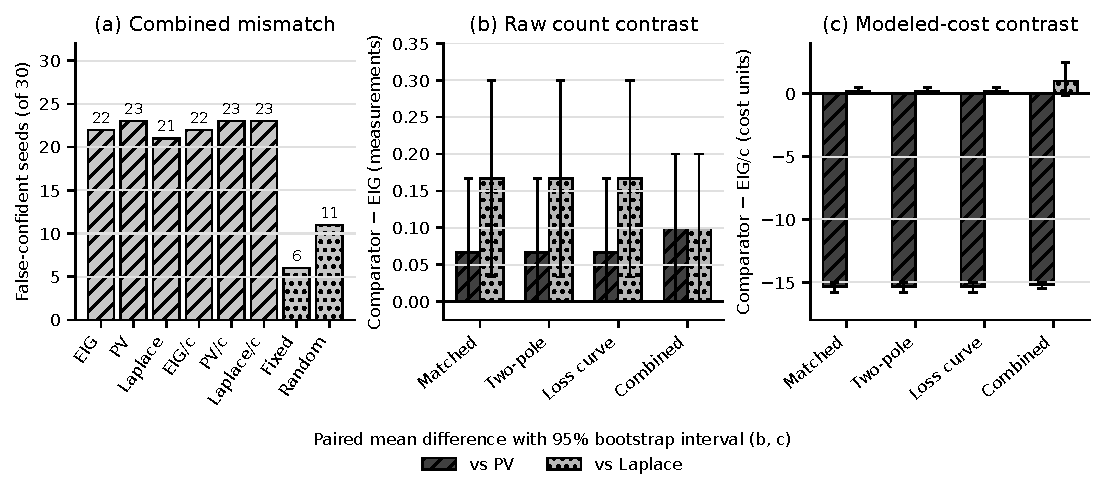
\includegraphics[width=\textwidth,height=0.38\textheight,keepaspectratio]{assets/model-mismatch-v3.pdf}
\caption{Controlled-mismatch results. Bars and error bars show paired
mean differences and descriptive 95\% paired-bootstrap intervals without
multiplicity adjustment; positive differences favor EIG. The /c policy
suffix denotes prespecified modeled cost, not measured laboratory time.
Combined-mismatch false-confidence counts are descriptive, not a causal
comparison among policies.}
\end{figure*}

\hypertarget{measured-data-model-adequacy}{%
\subsection{Measured-data model
adequacy}\label{measured-data-model-adequacy}}

For LEA Material Database permeability records that satisfied the
convergence criteria, RRMSEs were 9.33\%/52.42\% for \(\mu'/\mu''\) on
N87 and 6.89\%/36.77\% on N95. The larger \(\mu''\) errors expose
discrepancy in the one-pole model. N87 and 3C95 MagNet records failed
convergence or boundary gates and were excluded from numerical
claims~\citep{magnet2022}. Measured Steinmetz fits produced in-sample
RRMSEs of 8.79\% (N87), 12.55\% (N49), 13.40\% (3C95), and 18.21\% (N95)
within their specified temperature cohorts. These are fit residuals, not
held-out errors.
\href{https://github.com/hoangduong6210/EIG-bayesian-for-Recover-potential-Physical-Parameter-of-MagComponent/blob/927bbcb6d0b862598fae87d2575a872bbd79b5f1/wiki/evidence/Evidence-Sources.md\#e7}{Result
source E7}

\begin{figure*}[t]
\centering
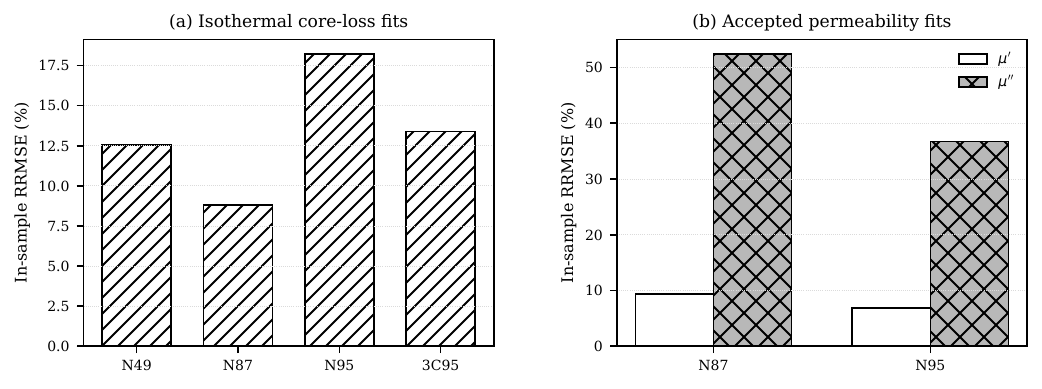
\includegraphics[width=\textwidth,height=0.38\textheight,keepaspectratio]{assets/measured-adequacy.png}
\caption{In-sample measured-data adequacy, with storage and loss
permeability reported separately.}
\end{figure*}

Each result family uses its declared models, data filters, seeds, and
evaluation criteria; the mismatch sampler and holdout differ explicitly
from those of the earlier matched-model comparison.

\hypertarget{discussion-and-limitations}{%
\section{Discussion and Limitations}\label{discussion-and-limitations}}

\hypertarget{interpretation-of-the-evidence}{%
\subsection{Interpretation of the
evidence}\label{interpretation-of-the-evidence}}

The framework separates whether available measurements constrain
parameters within a chosen model from whether that model represents
measured material behavior. Fisher information and posterior width
address the former locally or conditionally; reported in-sample
residuals expose, but do not fully quantify, the latter. The disjoint
synthetic holdout now measures latent prediction within the matched
family; held-out validation on independently acquired physical material
is not established by these results.

The synthetic results support implementation-level conclusions. Full
local rank shows that every active coordinate affects the specified
synthetic experiment, while the broad spectrum shows that those effects
occur at very different scales. The recovery table then checks the
nonlinear posterior under matched truth. Neither result implies that the
same coordinates are uniquely physical when the material response lies
outside the six-parameter family. This distinction matters for converter
models because several parameter sets can produce similar loss or
permeability over a narrow operating window yet diverge when frequency,
flux density, or temperature changes.

The paired acquisition result shows that EIG exploited posterior
structure relative to the fixed traversal, but it does not isolate an
EIG-specific advantage: raw predictive variance and Laplace D-optimality
reached the same gate in the same number of measurements. Under the
modeled-cost objective, predictive variance was better than EIG in every
seed. The result means only that these policies narrow two specified
latent-response intervals efficiently inside the matched model. It does
not establish accurate recovery of a physical component, global
predictive accuracy, or robustness to model misspecification.
\href{https://github.com/hoangduong6210/EIG-bayesian-for-Recover-potential-Physical-Parameter-of-MagComponent/blob/927bbcb6d0b862598fae87d2575a872bbd79b5f1/wiki/evidence/Evidence-Sources.md\#e4}{Contrast
source E4}

MM-3 sharpens this boundary. The local width gate remained easy to
satisfy under the locked discrepancy terms, while truth accuracy and
fixed latent- holdout inclusion deteriorated. In combined mismatch, raw
EIG was false- confident in 22 of 30 seeds, yet the other strong
adaptive policies produced similar counts. Model adequacy and
stopping-rule design therefore affected the interpretation more than the
small between-policy count differences. This is evidence about the three
registered departures, not a theorem for arbitrary misspecification.
\href{https://github.com/hoangduong6210/EIG-bayesian-for-Recover-potential-Physical-Parameter-of-MagComponent/blob/927bbcb6d0b862598fae87d2575a872bbd79b5f1/wiki/evidence/Evidence-Sources.md\#e16}{Model-mismatch
source E16}

\hypertarget{why-the-strong-comparators-tie-or-win}{%
\subsection{Why the strong comparators tie or
win}\label{why-the-strong-comparators-tie-or-win}}

The raw count tie is a resolution property of the declared stopping
endpoint, not proof that the acquisition rules rank candidates
identically. After four total measurements, no paired seed under any of
the three raw policies had passed both gates. Raw EIG still failed the
\(L_m\) gate in 28 of 30 seeds; predictive variance still failed core
loss in 16 and \(L_m\) in 14; Laplace D-optimality still failed core
loss in 21 and \(L_m\) in 9. Each policy then completed the
complementary response information at measurement five, so the integer
count endpoint collapsed their different paths to the same value. Their
ordered sequences confirm the distinction: EIG and predictive variance
match in only 11 of 30 seeds, while EIG and Laplace D-optimality match
in only 2 of 30.
\href{https://github.com/hoangduong6210/EIG-bayesian-for-Recover-potential-Physical-Parameter-of-MagComponent/blob/927bbcb6d0b862598fae87d2575a872bbd79b5f1/wiki/evidence/Evidence-Sources.md\#e5}{Trajectory
source E5}

The per-cost loss has a different mechanism. At the shared
four-measurement state available in 22 paired seeds, the mean core-loss
interval half-width is 26.03\%, above its 8\% gate, while the mean
\(L_m\) half-width is 2.78\%, below its 5\% gate. EIG/cost nevertheless
ranks an additional 10 kHz \(L_m\) measurement first in 21 of those
states because its mean joint information-per-cost utility is 0.05282,
compared with 0.04390 for the high-leverage core-loss point. Predictive
variance/cost ranks that core-loss point first in all 22 states and
crosses both gates one measurement earlier.
\href{https://github.com/hoangduong6210/EIG-bayesian-for-Recover-potential-Physical-Parameter-of-MagComponent/blob/927bbcb6d0b862598fae87d2575a872bbd79b5f1/wiki/evidence/Evidence-Sources.md\#e5}{Trajectory
source E5}

Thus EIG/cost behaves consistently with its own objective, but that
objective is not expected cost-to-gate. The experiment asks whether a
global parameter- information utility is efficient for reaching two
local predictive-width thresholds; it is not guaranteed to be. A
gate-aligned utility must be preregistered and evaluated as a new
experiment rather than substituted into this frozen result after
observing the comparison.

\hypertarget{implications-for-converter-modeling}{%
\subsection{Implications for converter
modeling}\label{implications-for-converter-modeling}}

For a converter workflow, the posterior is most useful as a conditional
input to loss, inductance, and sensitivity calculations over the
specified operating region. Posterior draws can be propagated through a
component model instead of substituting one nominal coefficient set,
allowing a designer to determine whether parameter uncertainty
materially affects thermal or magnetic design margins. The Fisher
spectrum can motivate testing whether a new channel or a wider,
physically controlled excitation range would constrain a weak direction
more effectively than densifying the original sweep
~\citep{chaloner1995, atkinson2007}.

Measured residuals define a separate model-adequacy assessment. The
accepted core-loss fits show the error remaining after estimating
Steinmetz coefficients inside one temperature cohort. The much larger
loss-component permeability residuals show that a single Cole--Cole pole
cannot be treated as a broadband physical description for these records.
A component calculation that is sensitive to \(\mu''\) should therefore
retain an explicit discrepancy allowance or adopt a higher-order
permeability law before relying on posterior parameter width.
Conversely, a reasonable \(\mu'\) residual does not validate \(\mu''\),
because the two components occupy different numerical scales and
correspond to different design consequences.

The common evaluation protocol safeguards this interpretation by
preventing combination of a favorable recovery run, a figure from
another seed set, and a measured fit produced under different filters.
Fixed model settings, data selections, and random seeds also make it
possible to distinguish sampling variation from changes to the
computational experiment.

\hypertarget{threats-to-validity}{%
\subsection{Threats to validity}\label{threats-to-validity}}

Internal validity is limited by five synthetic recovery seeds and 30
paired acquisition seeds. Pairing controls differences in candidate
outcomes between policies. A prespecified convergence study compares
candidate ranks and downstream endpoints against a higher-budget
reference; finite nested Monte Carlo variance nevertheless remains.
Synthetic recovery is matched-model, and the observed interval-inclusion
count is too small to establish calibrated coverage.

The independent MM-3 seed set adds a controlled structural-mismatch
test, but only for one two-pole permeability departure, one
temperature/curvature loss departure, and their combination. Its 90\%
latent-holdout inclusion is a fixed- point summary, not simulation-based
calibration. Production records retain sampler checkpoint histories but
not full chains, so the stored convergence decision can be reconstructed
while autocorrelation and acceptance cannot be independently recomputed
without rerunning the locked source.
\href{https://github.com/hoangduong6210/EIG-bayesian-for-Recover-potential-Physical-Parameter-of-MagComponent/blob/927bbcb6d0b862598fae87d2575a872bbd79b5f1/wiki/evidence/Evidence-Sources.md\#e16}{Source
E16}

The policy comparison now includes deterministic and randomized balanced
traversals, predictive variance, and Laplace D-optimality. It does not
include a full nonlinear Fisher-greedy implementation, space-filling
designs, multi-step look-ahead, or learned adaptive policies. More
importantly, the direct results do not establish EIG dominance over the
strong comparators. Observation noise and geometry are fixed, and
estimator intervals are not total physical-uncertainty intervals.

Construct validity is limited by the low-order forward models and
available data. The Steinmetz relation is temperature independent, and
one Cole--Cole pole does not capture all ferrite relaxation, resonance,
or loss processes ~\citep{tsutaoka2003}. Measured errors are in-sample.
Public curves may also contain digitization, instrument, preprocessing,
and source-specific errors not represented by the likelihood. Excluding
convergence-invalid or boundary-active records prevents unsupported
aggregate claims but restricts the population represented by the
accepted subset.

External validity is confined to the specified channels, temperature
cohorts, excitation ranges, materials, and cost model. The measured-data
EIG ranking is a model-conditional acquisition suggestion, not a
validated optimal laboratory plan, particularly given the observed
\(\mu''\) discrepancy. Measurement-count reductions must not be
interpreted as laboratory-time savings because setup, settling,
calibration, rejection, and batch costs were not measured. The results
do not replace held-out validation, controlled multi-lot
characterization, switching-waveform experiments, or component
qualification. Those extensions require new experimental evidence rather
than broader interpretation of the present results.

The strong-comparator campaign already produced an important negative
result: EIG did not beat either strong raw policy in the matched-model
count comparison and lost the per-cost comparison with predictive
variance. Publishing this outcome prevents the favorable fixed-traversal
comparison from being generalized beyond its actual comparator.
\href{https://github.com/hoangduong6210/EIG-bayesian-for-Recover-potential-Physical-Parameter-of-MagComponent/blob/927bbcb6d0b862598fae87d2575a872bbd79b5f1/wiki/evidence/Evidence-Sources.md\#e4}{Sources
E4} and
\href{https://github.com/hoangduong6210/EIG-bayesian-for-Recover-potential-Physical-Parameter-of-MagComponent/blob/927bbcb6d0b862598fae87d2575a872bbd79b5f1/wiki/evidence/Evidence-Sources.md\#e5}{E5}

\hypertarget{conclusion}{%
\section{Conclusion}\label{conclusion}}

Bayesian calibration recovered the active Steinmetz and Cole--Cole
parameters with per-parameter median absolute relative errors of
0.27\%--5.85\% across five matched-model synthetic data sets; the
generating values lay within 28 of 30 model-conditional 90\% credible
intervals. Raw EIG reached the two-target precision gate in five
measurements rather than nine for the fixed traversal, but it tied
predictive variance and Laplace D-optimality in all 30 direct count
comparisons. EIG/cost tied Laplace D-optimality and lost to predictive
variance/cost by a mean 15.17 modeled-cost units. The accepted measured
records produced substantially larger RRMSE for \(\mu''\) than for
\(\mu'\), showing that posterior concentration cannot compensate for an
inadequate permeability law. MM-3 reinforces that conclusion
synthetically: combined-mismatch raw EIG reached the precision gate in
every seed but was false-confident in 22 of 30, while its count
advantage over either strong comparator was only 0.10 measurements. The
local gate is therefore not evidence of truth accuracy under the locked
structural departures. The defensible conclusion is therefore a
reproducible model-conditional benchmark with informative positive and
negative results, not proof of EIG superiority or laboratory efficiency.
\href{https://github.com/hoangduong6210/EIG-bayesian-for-Recover-potential-Physical-Parameter-of-MagComponent/blob/927bbcb6d0b862598fae87d2575a872bbd79b5f1/wiki/evidence/Evidence-Sources.md\#e2}{Evidence
E2},
\href{https://github.com/hoangduong6210/EIG-bayesian-for-Recover-potential-Physical-Parameter-of-MagComponent/blob/927bbcb6d0b862598fae87d2575a872bbd79b5f1/wiki/evidence/Evidence-Sources.md\#e4}{E4},
\href{https://github.com/hoangduong6210/EIG-bayesian-for-Recover-potential-Physical-Parameter-of-MagComponent/blob/927bbcb6d0b862598fae87d2575a872bbd79b5f1/wiki/evidence/Evidence-Sources.md\#e7}{E7},
and
\href{https://github.com/hoangduong6210/EIG-bayesian-for-Recover-potential-Physical-Parameter-of-MagComponent/blob/927bbcb6d0b862598fae87d2575a872bbd79b5f1/wiki/evidence/Evidence-Sources.md\#e16}{E16}

\hypertarget{exact-sequential-evaluation-logic}{%
\section{Exact Sequential Evaluation
Logic}\label{exact-sequential-evaluation-logic}}

For each confirmatory seed, the synthetic truth is drawn once from the
fixed prior. One outcome per exact candidate identity is then generated
and stored. Each policy is evaluated by the following logic:

\begin{enumerate}
\def\labelenumi{\arabic{enumi}.}
\item
  Start with the same declared \(P_v\) and \(\mu'\) observations.
\item
  Fit the six-coordinate posterior and require all sampler gates.
\item
  If both target intervals satisfy the precision gate, retain count and
  modeled cost and stop successfully.
\item
  Otherwise score or traverse only unrevealed candidates. EIG uses
  \(\widehat U(d)\); predictive variance uses noise-normalized posterior
  response variance; Laplace D-optimality uses the log-determinant
  precision increment. Per-cost forms divide by \(c(d)\). Fixed and
  randomized policies follow their declared channel-balanced traversals.
\item
  Break deterministic ties by exact design identity, reveal the stored
  outcome for the selected identity, append it, and return to step 2.
\item
  If the 25-measurement budget is exhausted, retain the trajectory as a
  failure rather than imputing a stopping count.
\end{enumerate}

This logic separates three random objects: the prior-predictive truth,
the candidate-indexed outcome table, and the policy's numerical scoring
stream. Changing policy order changes neither the truth nor any
candidate outcome. Stable design identities also make EIG scores
invariant to permutation of the input library.

\hypertarget{endpoint-and-uncertainty-definitions}{%
\section{Endpoint and Uncertainty
Definitions}\label{endpoint-and-uncertainty-definitions}}

For a latent target \(g(\theta)\), the reported precision statistic is
\[h_g=100\,\frac{q_{0.95}[g(\theta)]-q_{0.05}[g(\theta)]}
 {2\,|q_{0.50}[g(\theta)]|}.\] The gate requires \(h_{P_v}\leq8\) and
\(h_{L_m}\leq5\). The measurement-count endpoint is the number of
revealed observations, including the two initial points, at the first
satisfied gate. The cost endpoint is the sum of declared channel costs
through that same step. Because the cost constants were not measured,
the endpoint is dimensionless modeled burden even though the
configuration names them as seconds for engineering convenience.

For paired seed \(s\) and a declared direct comparator, the endpoint
difference is comparator minus EIG, so a positive value favors EIG.
Resampling is performed over complete paired seeds, never over unpaired
policy outcomes. Monte Carlo score intervals come from repeated
estimates of the nested estimator; posterior intervals come from
retained sampler draws; paired bootstrap intervals come from the 30
seed-level differences. These three intervals answer different questions
and are not interchangeable.

\hypertarget{evidence-and-software-availability}{%
\section{Evidence and software
availability}\label{evidence-and-software-availability}}

Numerical results are bound to validated scientific freeze
\texttt{20260817T072230Z\_401e3030fe13}, manifest SHA-256
\texttt{85448a2c\allowbreak{}3c9db2db\allowbreak{}051c9454\allowbreak{}3d8a336e\allowbreak{}7157d552\allowbreak{}89f10c17\allowbreak{}92e9c57d\allowbreak{}433812f7}.
The freeze contains the 30 complete eight-policy trajectories, estimator
states and scores, point-level 23-point holdouts, parameter-recovery
records, and reconstructed endpoints. The sanitized v2 public audit
bundle is available as a versioned release asset. The public bundle
omits machine-specific operational metadata. Raw measured curves remain
governed by the cited upstream sources and are not redistributed as if
produced by this study.
\href{https://github.com/hoangduong6210/EIG-bayesian-for-Recover-potential-Physical-Parameter-of-MagComponent/blob/927bbcb6d0b862598fae87d2575a872bbd79b5f1/wiki/evidence/Evidence-Sources.md\#e8}{Release
source E8}

The separate MM-3 result is bound to aggregate SHA-256
\texttt{03e8d81c\allowbreak{}48f3b5eb\allowbreak{}2c807a47\allowbreak{}b880972d\allowbreak{}3ea727b1\allowbreak{}49788c2d\allowbreak{}effc35f1\allowbreak{}ac1d222d}.
Its public audit asset contains all 120 sanitized task records and
reconstructs the aggregate; it omits full walker-by-iteration chains.
\href{https://github.com/hoangduong6210/EIG-bayesian-for-Recover-potential-Physical-Parameter-of-MagComponent/blob/927bbcb6d0b862598fae87d2575a872bbd79b5f1/wiki/evidence/Evidence-Sources.md\#e16}{Model-mismatch
source E16}

The
\href{https://github.com/hoangduong6210/EIG-bayesian-for-Recover-potential-Physical-Parameter-of-MagComponent/blob/927bbcb6d0b862598fae87d2575a872bbd79b5f1/wiki/results/Scientific-Job-Results.md}{scientific
job ledger} accounts for every result artifact in the release, and
\href{https://github.com/hoangduong6210/EIG-bayesian-for-Recover-potential-Physical-Parameter-of-MagComponent/blob/927bbcb6d0b862598fae87d2575a872bbd79b5f1/wiki/evidence/Evidence-Sources.md}{Evidence
Sources} maps each quantitative result family to an exact pointer in the
disclosure-safe projection.
